\documentclass{beamer}
\usepackage[latin1]{inputenc}
%\usetheme{Montpellier}
%\usetheme{Boadilla}
%\usecolortheme[RGB={204,51,255}]{structure}
%\usecolortheme[named=purple]{structure}
\usecolortheme[RGB={128,62,62}]{structure}
%\definecolor{dark}{rgb}{0.3,0.15,0.3}
%\definecolor{light}{rgb}{0.8,0.6,0.8}
%\definecolor{reddish}{rgb}{.5,0.15,0.15}
\definecolor{dark}{rgb}{0.5,0.3,0.4}
%\definecolor{light}{rgb}{0.8,0.6,0.8}
\definecolor{reddish}{rgb}{.7,0.25,0.25}
\definecolor{greenish}{rgb}{.25,0.7,0.25}
\definecolor{blueish}{rgb}{.25,0.25,0.7}
\definecolor{purple}{rgb}{.5,0.0,0.5}
\usepackage{graphicx}
\usepackage{pstricks}

\usepackage{amssymb}

\usepackage{amsmath}
\setbeamertemplate{navigation symbols}{}

\newcommand{\crish}{\color{reddish}}
\newcommand{\cbla}{\color{black}}
\newcommand{\cred}{\color{red}}
\newcommand{\cblu}{\color{blue}}

\newcommand{\sm}{\color{reddish}$}
\newcommand{\fm}{$\color{black}}
\usepackage{tikz}
\usetikzlibrary{arrows,decorations.markings,positioning}
\usetikzlibrary{calc,fit,shapes, backgrounds} 

\usepackage{epstopdf}
\title{Lecture 8: Conditional Independance}
\author{COMS10014 Mathematics for Computer Science A}
\institute{\texttt{cs-uob.github.io/COMS10014/ and github.com/coms10011/2020\_21}}
\date{November 2020}
\begin{document}

\maketitle

\begin{frame}{Independent Events}
Two events   \crish$A$\cbla{} and   \crish$B$\cbla{} are \textbf{independent} iff 
  \crish$$P(A|B)=P(A)$$\cbla{}
\end{frame}
\begin{frame}{Independent Events}
  Recall
  \crish$$P(A\cap{} B)=P(A|B)P(B)$$\cbla{}
so  \crish$A$\cbla{} and   \crish$B$\cbla{} are \textbf{independent} iff 
  \crish$$P(A\cap{} B)=P(A)P(B)$$\cbla{}
\end{frame}

\begin{frame}{Snakes and Ladders or Moksha Patam}
  \begin{center}
    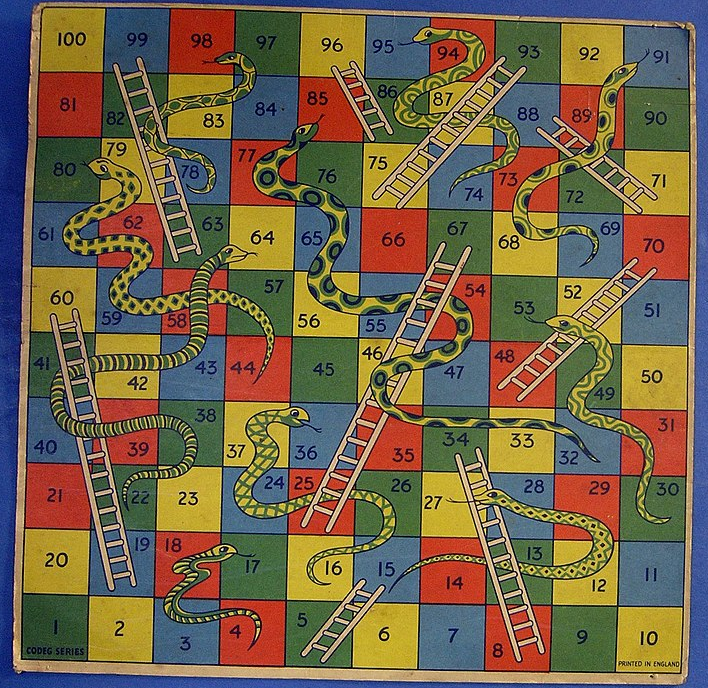
\includegraphics[width=8cm]{game.png}
  \end{center}
    \vfill
\tiny{\flushright{Image from wikipedia.}}
\end{frame}


\begin{frame}{start at 1}
  \begin{center}
    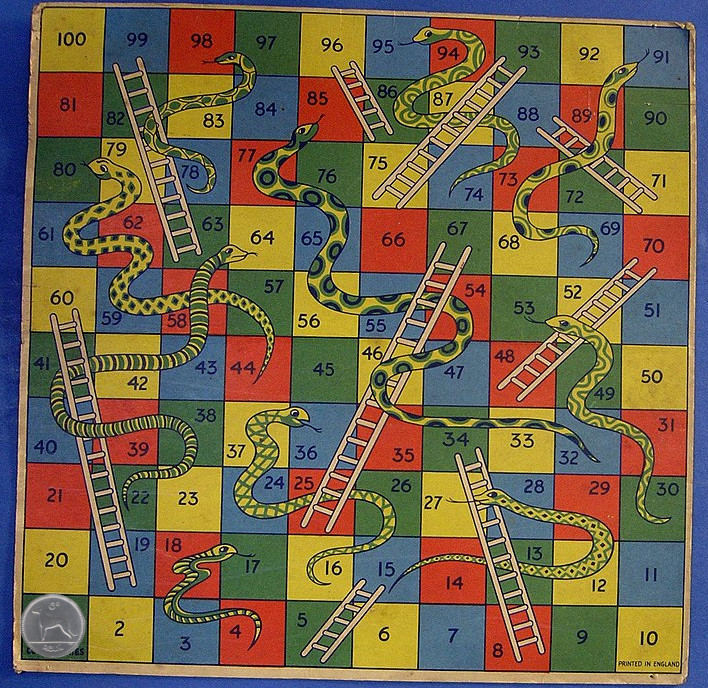
\includegraphics[width=8cm]{game1.jpg}
  \end{center}
    \vfill
\tiny{\flushright{Image from wikipedia.}}
\end{frame}


\begin{frame}{1$\rightarrow$5 (roll 4)}
  \begin{center}
    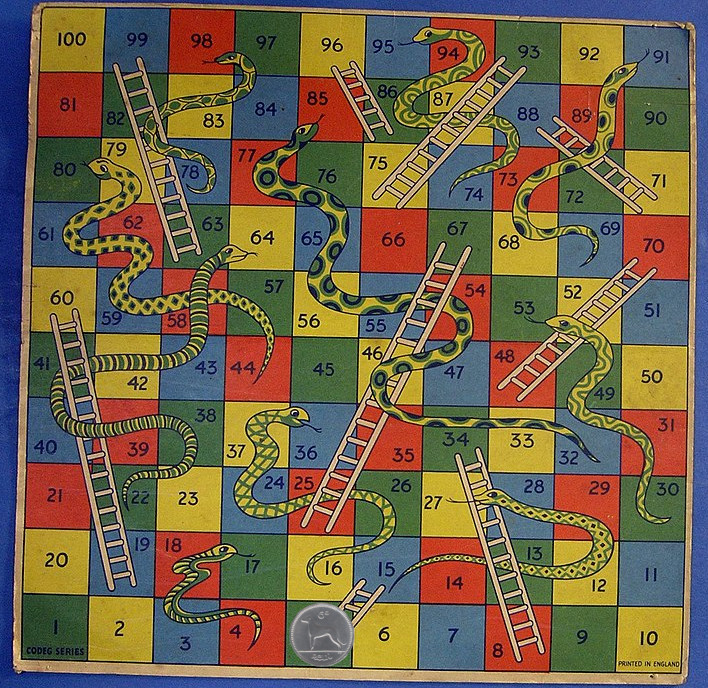
\includegraphics[width=8cm]{game5.jpg}
  \end{center}
    \vfill
\tiny{\flushright{Image from wikipedia.}}
\end{frame}


\begin{frame}{1$\rightarrow$15 (up the ladder)}
  \begin{center}
    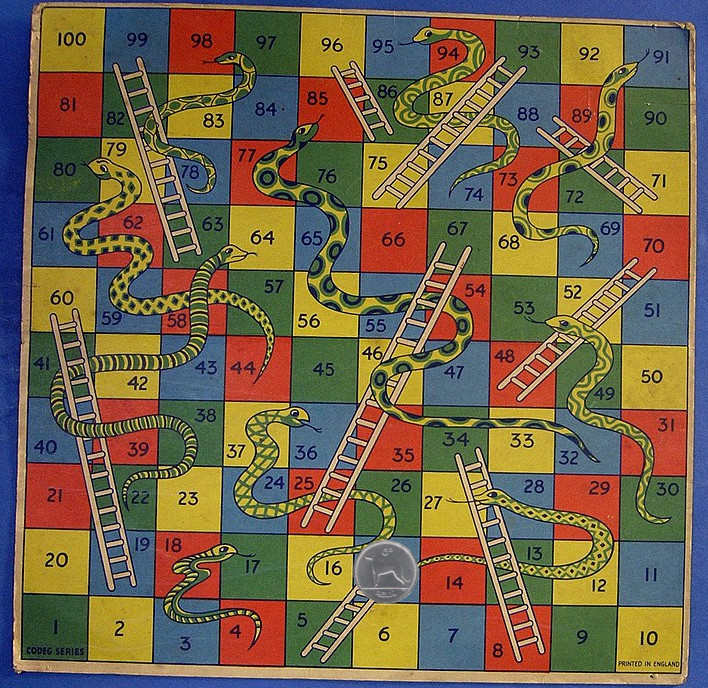
\includegraphics[width=8cm]{game15.jpg}
  \end{center}
    \vfill
\tiny{\flushright{Image from wikipedia.}}
\end{frame}


\begin{frame}{1$\rightarrow$15$\rightarrow$19 (roll another 4)}
  \begin{center}
    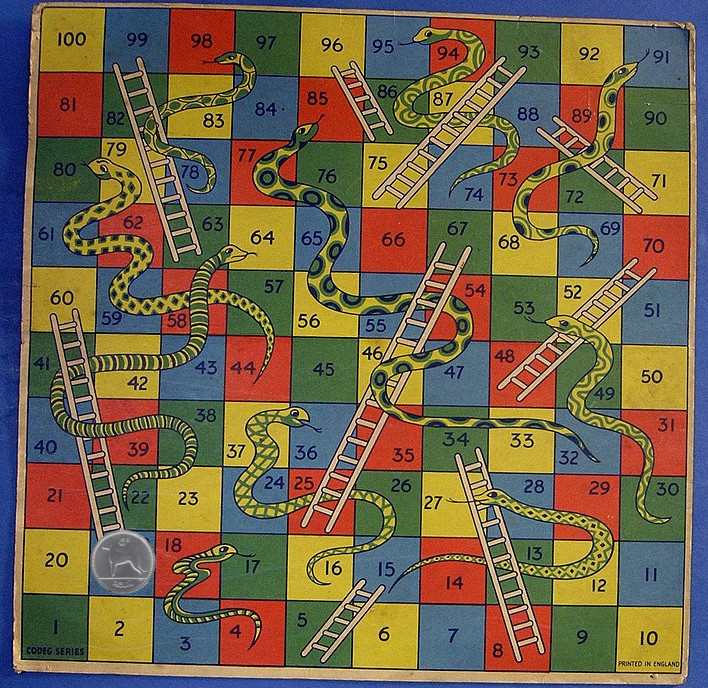
\includegraphics[width=8cm]{game19.jpg}
  \end{center}
    \vfill
\tiny{\flushright{Image from wikipedia.}}
\end{frame}


\begin{frame}{1$\rightarrow$15$\rightarrow$19$\rightarrow$60 (up the ladder)}
  \begin{center}
    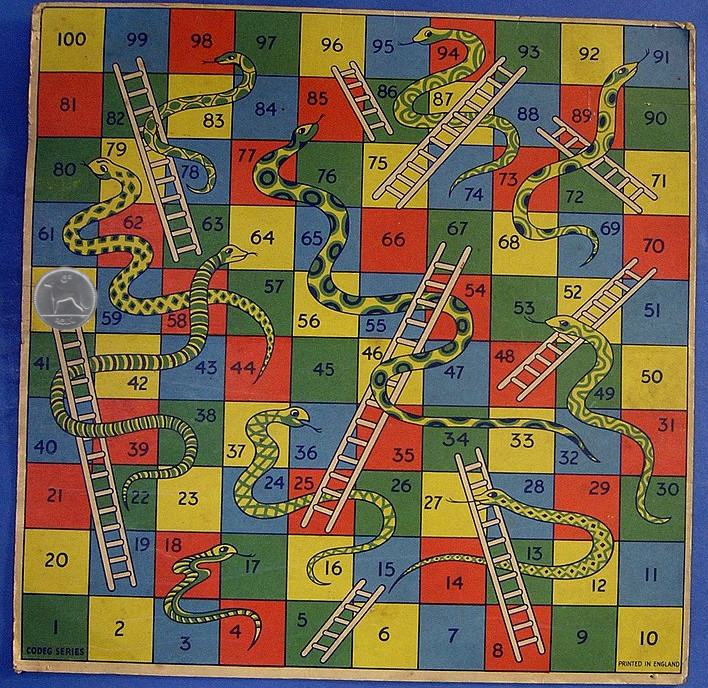
\includegraphics[width=8cm]{game60.jpg}
  \end{center}
    \vfill
\tiny{\flushright{Image from wikipedia.}}
\end{frame}


\begin{frame}{1$\rightarrow$15$\rightarrow$19$\rightarrow$60$\rightarrow$63 (roll a 3)}
  \begin{center}
    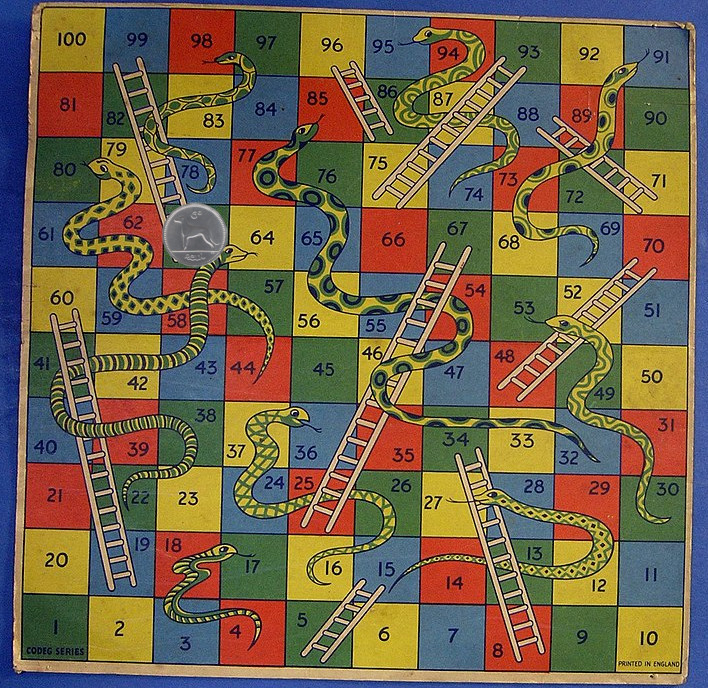
\includegraphics[width=8cm]{game63.jpg}
  \end{center}
    \vfill
\tiny{\flushright{Image from wikipedia.}}
\end{frame}


\begin{frame}{1$\rightarrow$15$\rightarrow$19$\rightarrow$60$\rightarrow$63$\rightarrow$99 (up the ladder)}
  \begin{center}
    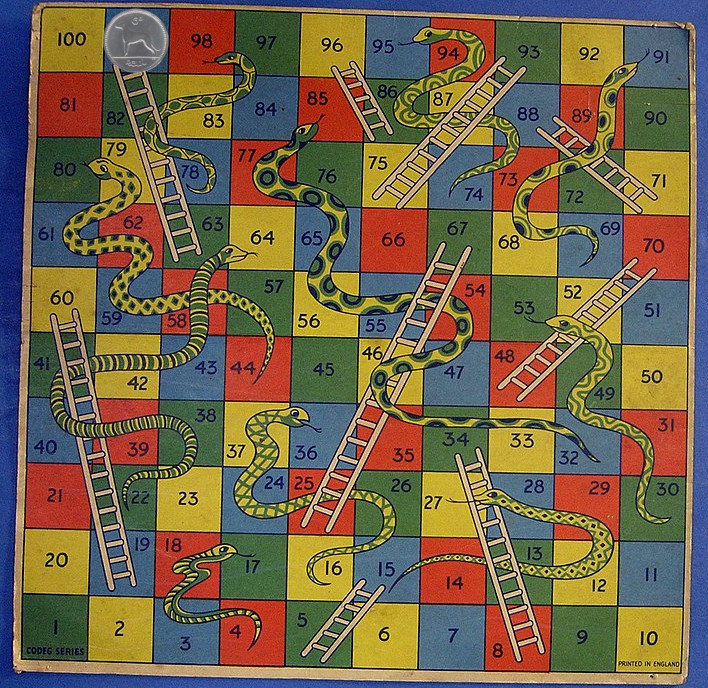
\includegraphics[width=8cm]{game99.jpg}
  \end{center}
    \vfill
\tiny{\flushright{Image from wikipedia.}}
\end{frame}


\begin{frame}{(4,4,3)}
  \begin{center}
    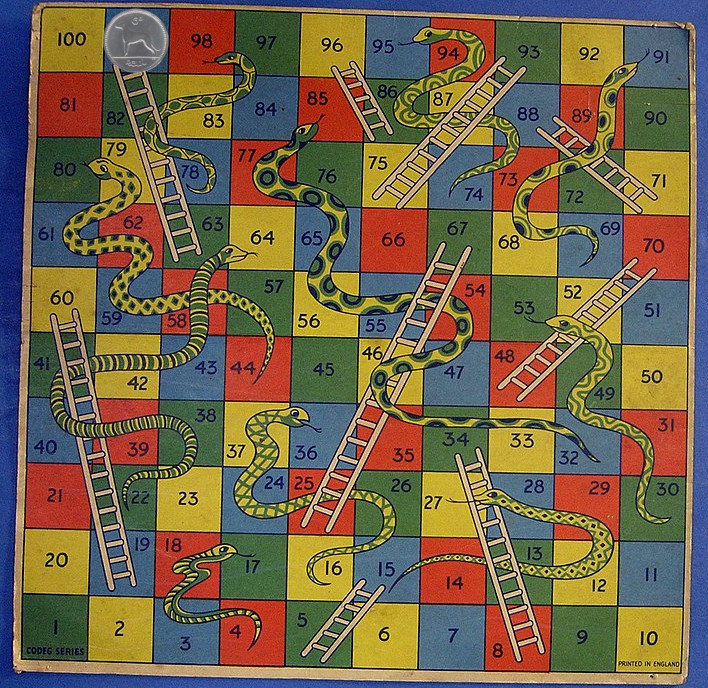
\includegraphics[width=8cm]{game99.jpg}
  \end{center}
    \vfill
\tiny{\flushright{Image from wikipedia.}}
\end{frame}


\begin{frame}{()}
  \begin{center}
    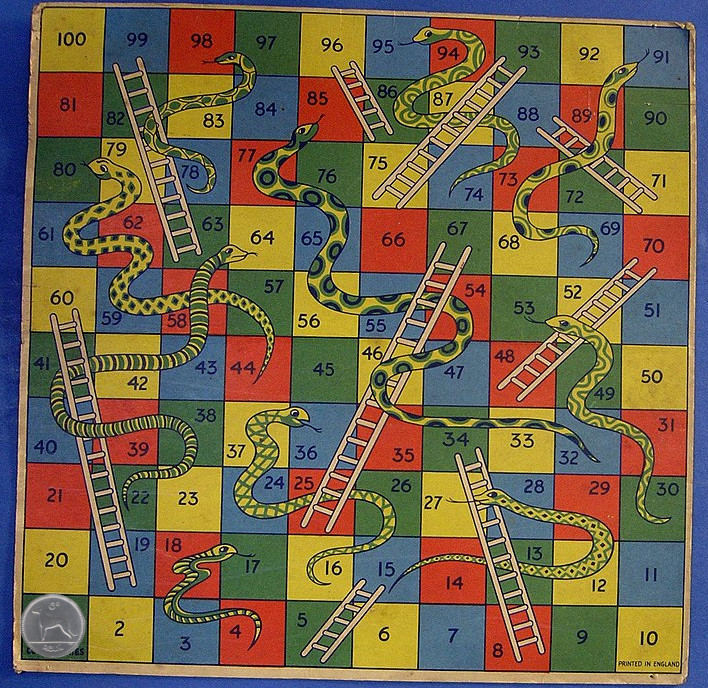
\includegraphics[width=8cm]{game1.jpg}
  \end{center}
    \vfill
\tiny{\flushright{Image from wikipedia.}}
\end{frame}


\begin{frame}{(8)}
  \begin{center}
    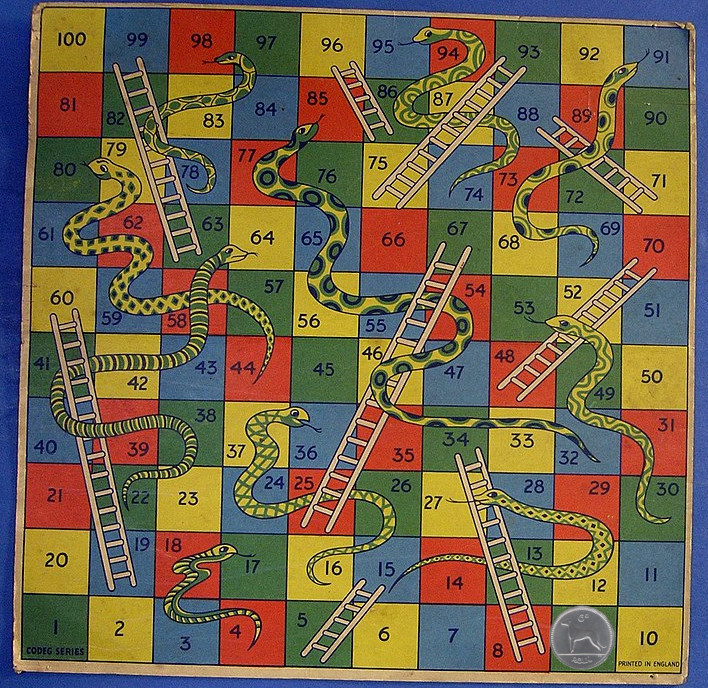
\includegraphics[width=8cm]{game9.jpg}
  \end{center}
    \vfill
\tiny{\flushright{Image from wikipedia.}}
\end{frame}


\begin{frame}{(8,10)}
  \begin{center}
    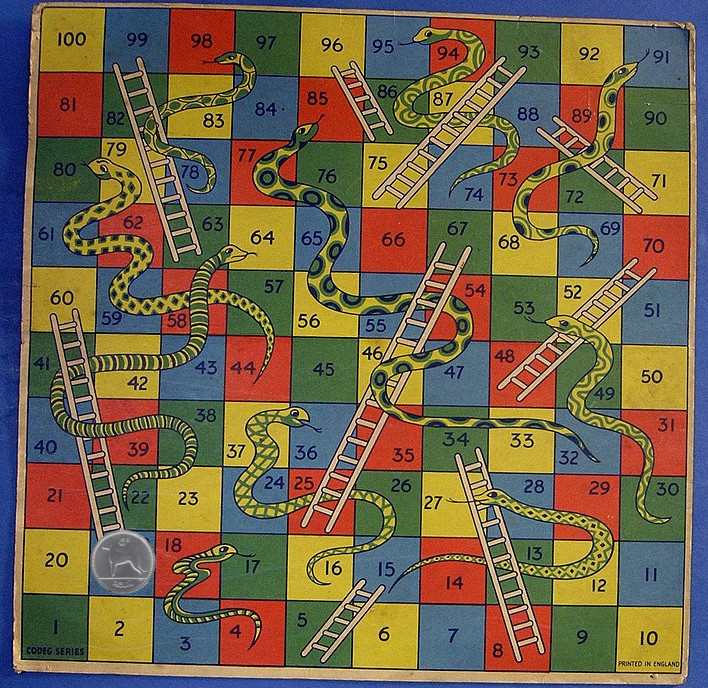
\includegraphics[width=8cm]{game19.jpg}
  \end{center}
    \vfill
\tiny{\flushright{Image from wikipedia.}}
\end{frame}


\begin{frame}{(8,10)}
  \begin{center}
    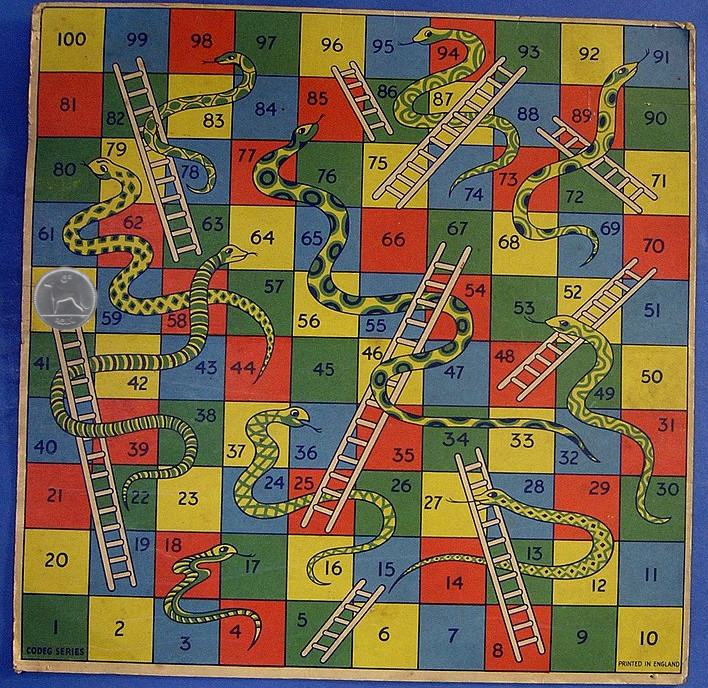
\includegraphics[width=8cm]{game60.jpg}
  \end{center}
    \vfill
\tiny{\flushright{Image from wikipedia.}}
\end{frame}


\begin{frame}{(8,10,3)}
  \begin{center}
    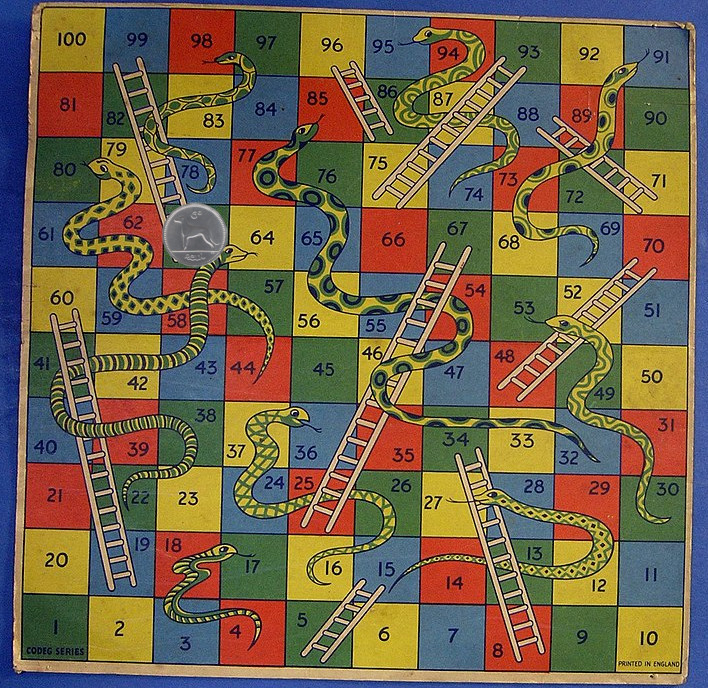
\includegraphics[width=8cm]{game63.jpg}
  \end{center}
    \vfill
\tiny{\flushright{Image from wikipedia.}}
\end{frame}


\begin{frame}{(8,10,3)}
  \begin{center}
    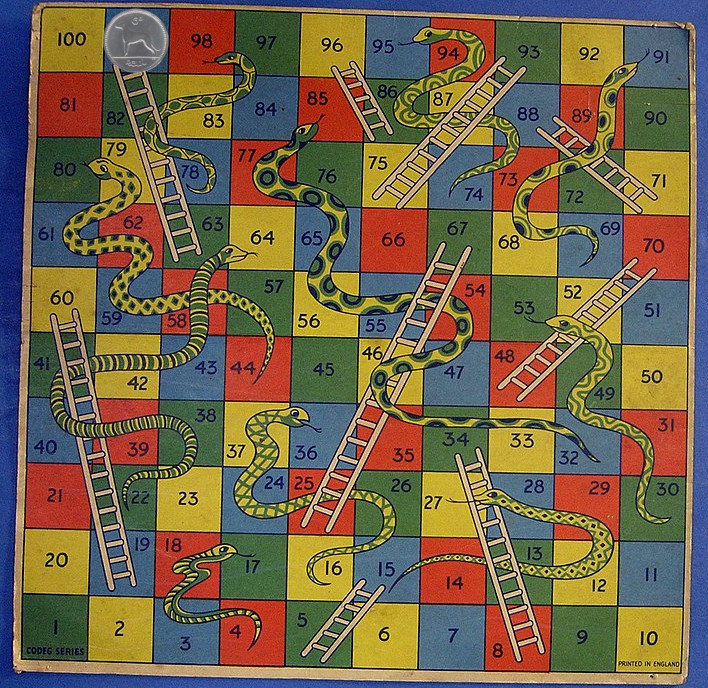
\includegraphics[width=8cm]{game99.jpg}
  \end{center}
    \vfill
\tiny{\flushright{Image from wikipedia.}}
\end{frame}

\begin{frame}{Probability}
\begin{itemize}
\item \crish $Xn$\cbla, at place \crish$n$\cbla{} end of the first move,
\item \crish $Yn$\cbla,  at place \crish$n$\cbla{} end of the second move,
\item \crish$Zn$\cbla{},  at place \crish$n$\cbla{} end of the third move,
\end{itemize}  
after doing all the snakes and ladders stuff.
\vskip 1cm So \crish$Z99$\cbla{} is the event of getting to 99 at the
end of the third move.
\end{frame}

\begin{frame}{Probability}
  \crish $$ P(Z99)=0.0031 $$ \cbla
  You can work this out by adding
  \crish
  \begin{eqnarray*}    
  P(Z99)&=&P(Z99|Y60\cap{}X15)P(Y60|X15)P(X15)\cr&&+P(Z99|Y60\cap{}X13)P(Y60|X13)P(X13)+\ldots\end{eqnarray*}\cbla{}
\end{frame}

\begin{frame}{Conditional probability - rolling a four}
    \crish $$ P(Z99|X15)=0.0046 $$ \cbla
  \begin{center}
    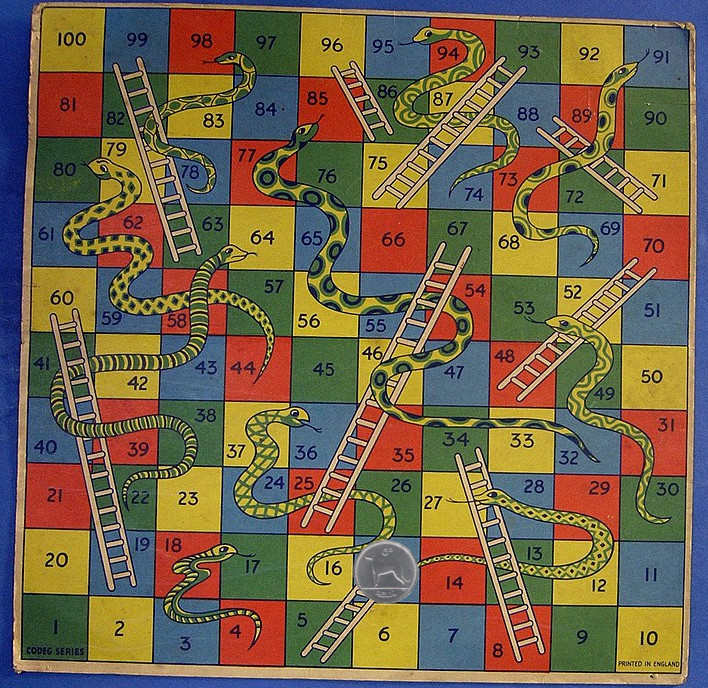
\includegraphics[width=7cm]{game15.jpg}
  \end{center}
\end{frame}


\begin{frame}{Probability}
  \crish $$ P(Z99)\not=P(Z99|X15) $$ \cbla
\end{frame}


\begin{frame}{Conditional probability - rolling an eight}
    \crish $$ P(Z99|X9)=0.0046 $$ \cbla
  \begin{center}
    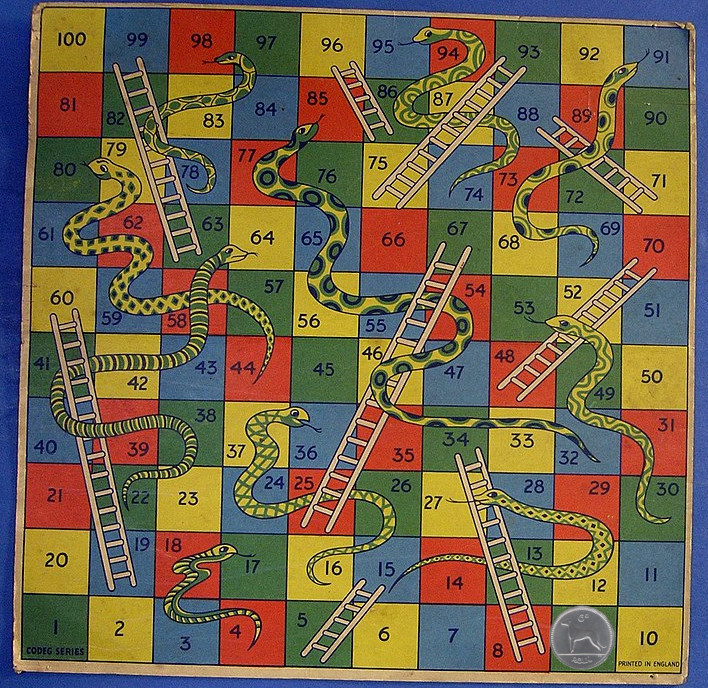
\includegraphics[width=7cm]{game9.jpg}
  \end{center}
\end{frame}


\begin{frame}{Conditional probability - rolling a 12}
    \crish $$ P(Z99|X13)=0.0077 $$ \cbla
  \begin{center}
    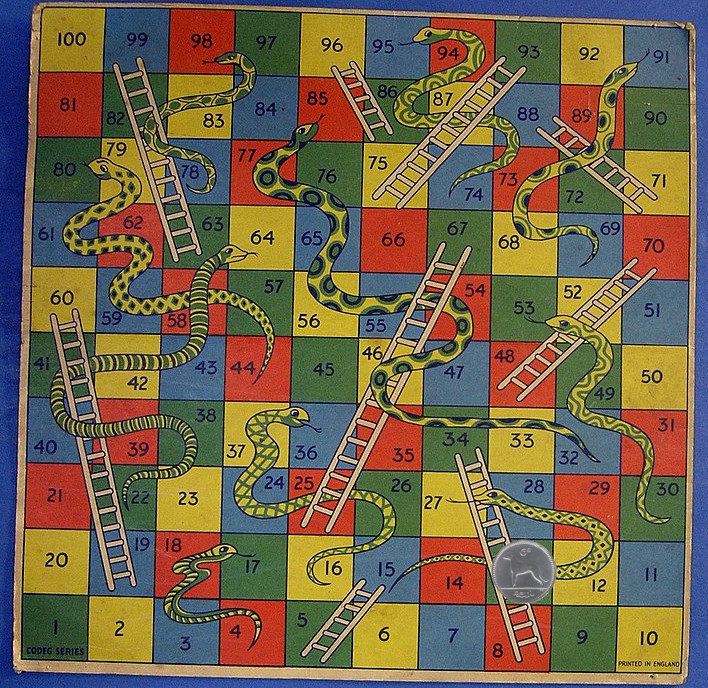
\includegraphics[width=7cm]{game13.jpg}
  \end{center}
\end{frame}

\begin{frame}{Conditional probability - rolling a seven}
    \crish $$ P(Z99|X34)=0 $$ \cbla
  \begin{center}
    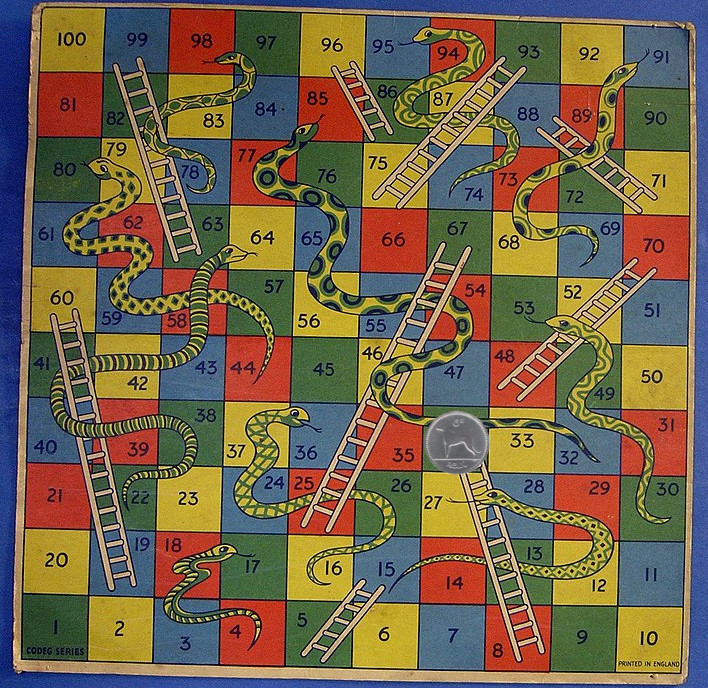
\includegraphics[width=7cm]{game34.jpg}
  \end{center}
\end{frame}


\begin{frame}{Conditional probability - getting to 60}
    \crish $$ P(Z99|Y60)=0.0556 $$ \cbla
  \begin{center}
    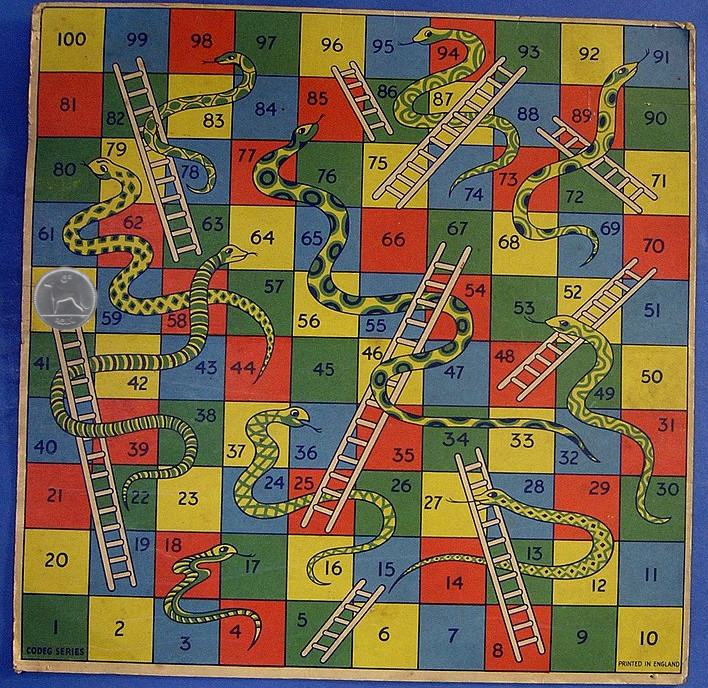
\includegraphics[width=7cm]{game60.jpg}
  \end{center}
\end{frame}

\begin{frame}{Conditional probability - \crish$X$\cbla{} no longer matters}
    \crish $$ P(Z99|Y60)=P(Z99|Y60\cap{}X15) $$ \cbla
  \begin{center}
    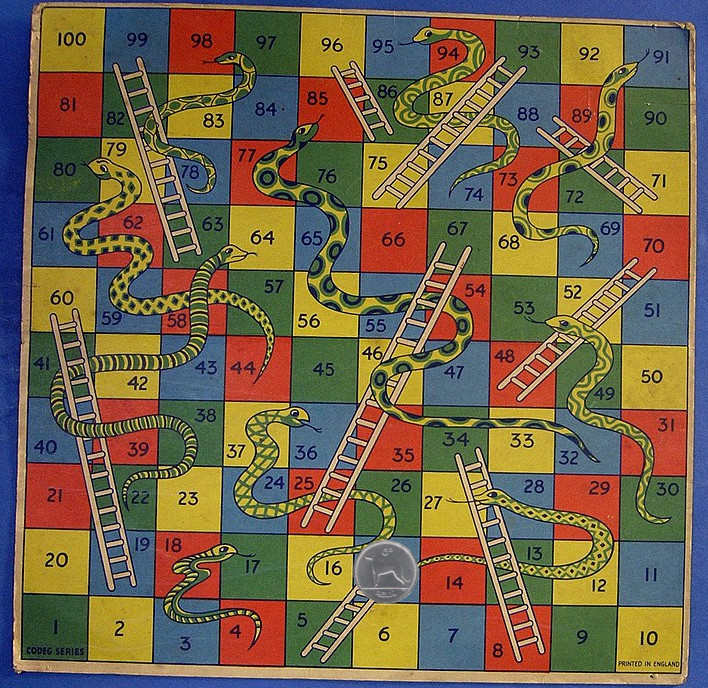
\includegraphics[width=7cm]{game15.jpg}
  \end{center}
\end{frame}


\begin{frame}{Conditional probability - \crish$X$\cbla{} no longer matters}
  \crish $$ P(Z99|Y60)=P(Z99|Y60\cap{}X10) $$ \cbla
    \begin{center}
    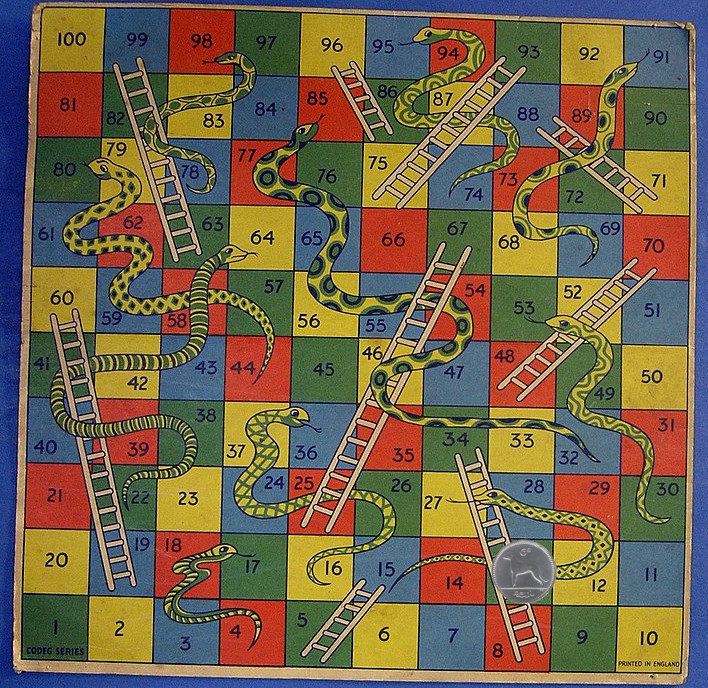
\includegraphics[width=7cm]{game13.jpg}
  \end{center}
\end{frame}


\begin{frame}{Conditional independence}
\crish$X$\cbla{} and \crish$Z$\cbla{} are conditionally independent:
\crish
$$
P(Xn_1\cap{}Zn_3|Yn_2)=P(Xn_1|Yn_2)P(Zn_3|Yn_2)
$$
\cbla
\end{frame}

\begin{frame}{Conditional independence}
  \crish$A$\cbla{} and  \crish$C$\cbla{} and \textbf{conditionally independent} given \crish$C$\cbla{} if
  \crish$$P(A\cap{}C|B)=P(A|B)P(C|B)$$\cbla{}
  \end{frame}



\end{document}

